\section{Learning seed bounds from complete reduction time}
\label{sec:learned-bounds}
The broader test found that the earlier models often kept native choices and provided little additional benefit. We therefore train a new model for a decision that directly changes equation generation: the seed limits for the requested target batch. The model chooses these limits before Kira starts. All earlier seed, row, and equation models are disabled in this comparison, and every method uses the same exact preparation. The fixed-control comparison measures the extra benefit of a learned choice after tuning the seed settings.

\subsection{What the model learns and how Kira uses it}
A target batch can need a larger numerator bound even when its denominators require no further increase. Other batches can use fewer seeds in lower sectors. Kira provides bounds on positive powers, numerator rank, and extra denominator powers, as well as a separate restriction for lower sectors~\cite{Kira3}. These settings define ten candidate configurations in the present study. They include unshifted bounds, selective expansion, reduced bounds, full expansion, and four configurations with lower sector truncation. Appendix~\ref{app:learned-bounds} specifies every configuration and its recovery sequence.

The model receives 27 quantities that describe the graph and target indices. For each target $\boldsymbol a$, the extra denominator powers are $\delta(\boldsymbol a)=\sum_i\max(a_i-1,0)$, and the numerator rank is $\rho(\boldsymbol a)=\sum_i\max(-a_i,0)$. The first sum counts denominator powers beyond one, often called dots, and the second is the total numerator power. Together with the loop count and denominator structure, these quantities help the model predict the relative complete time of each configuration. Its training labels come from actual Kira reductions, including any failed first attempt and the subsequent recovery. The prediction therefore concerns the cost of reaching a checked answer, rather than the number of selected seeds alone. Related work uses learned search to discover sparse seed patterns~\cite{Song2025,TubeSeeding2026}; the present experiment uses Kira's existing seed-region controls and does not implement tube seeding. The application checks the ordered momentum structure and the target-count and overall index-power ranges recorded in training and validation. Inputs outside this domain use native bounds and the same exact recovery procedure.

We compare 30 fitted models: regression trees, random forests, extremely randomized trees, and multilayer perceptrons~\cite{CART1984,Breiman2001Forest,Geurts2006ExtraTrees,Pedregosa2011Bounds}. Each model predicts ten costs. Validation selects a random forest with a gate on predicted log cost of 0.0. The selected predictor uses 48 trees, maximum depth 8, and at least 2 training cases per leaf. The model receives no reference coefficients, case identifier, or kinematic profile number. Its inputs and fitted parameters remain fixed during the reserved test. Details of the objective, model choices, and selection rule appear in Appendix~\ref{app:learned-bounds}.

For each request, the application loads the fitted parameters, calculates the features, and selects a configuration. Kira then generates IBP equations and performs exact algebra in the supplied master basis. If the chosen seed region cannot reach that basis, the application tries the unshifted bounds and then full expansion, skipping duplicate configurations. A request that exhausts these attempts remains unsuccessful. Coefficient comparisons occur after Kira has produced its result and are included in the reported time.

\subsection{Independent inputs and controls}
The input grid contains ten graph structures at one through four loops, with one to three target integrals per batch. It includes vacuum and two-point integrals, planar and nonplanar boxes, a pentagon, a box with an external virtuality, and boxes with bubble subgraphs. We define 74 training requests, 37 validation requests, and 74 reserved requests at separate rational kinematic profiles, keeping the dimension symbolic. After reference checks, complete candidate comparisons, and removal of identity-only cases, 68 training batches and 34 validation batches supply the fitted comparison. Target positions change with the profile, but graph structures and target patterns are shared. This tests transfer to new requests within known structures, not arbitrary new topologies or general symbolic kinematics.

Each reserved request first receives a reference reduction and a second exact check with a larger numerator bound. These preparation calculations provide a common basis and comparison coefficients. Agreement after one enlarged seed region does not prove that this basis has the smallest possible size. They remain outside the timed application, whose purpose is reduction in an available basis. The tests therefore include native IBP generation but do not include finding the master basis from the beginning. Some target patterns coincide when a family has no auxiliary numerator. Each declared batch remains a separate workload request, and the uncertainty calculation across graphs keeps such related requests together.

The first control uses Kira's native equation and elimination choices with the unshifted target bounds and the common expansion fallback. This is a specified seed policy, not a claim that Kira has a universal default seed region. The stronger fixed control chooses the cheapest of the same ten configurations separately for each graph, using both training and validation costs. It performs no model prediction and can use lower sector truncation. The learned method may change its choice between target batches in the same graph. All three methods use the same executable, exact optimizations, one Kira worker, basis, coefficient checks, and resource limits. Five repetitions rotate their order on the same node. The timer includes model loading, prediction, equation generation, exact elimination, retries, verification, and cleanup. Initial Python imports occur before this timer.

\subsection{Measured benefit and remaining limits}
Of the 74 reserved requests, 68 supply matched nontrivial reductions for all three methods and all repetitions. The record also contains 4 failed reference checks, 0 incomplete timed requests, and 2 matched identity-only requests. The full timed record contains 1050 exact completions in 1050 requests and 23295 coefficient comparisons. Failed or identity-only requests do not enter the paired speedup estimate.

Summing the median time of each matched batch gives 164.926 seconds for the control with native bounds, 119.717 seconds for the tuned fixed control, and 119.081 seconds for the learned choice. The learned method therefore takes 27.8\% less time than the control with native bounds and 0.5\% less time than the tuned fixed control. The corresponding speedup factors are 1.385 and 1.005. Table~\ref{tab:learned-bounds} gives the graph results, including slower groups. These are complete application-time comparisons on the same inputs; they are separate from the earlier exact-code speedups.

\begin{table}[!htbp]\centering\small
\caption{Sum of batch median times in seconds for the new seed-bound comparison. Every row uses matched nontrivial reductions. The fixed control uses one configuration per graph.}
\label{tab:learned-bounds}
\begin{tabular}{@{}lrrrrr@{}}\toprule
Graph & Loops & Batches & Native bounds & Fixed & Learned\\\midrule
Massive sunrise & 2 & 8 & 3.90 & 3.87 & 3.93\\
Planar double box & 2 & 8 & 15.22 & 13.56 & 13.40\\
Massive vacuum & 3 & 8 & 6.35 & 6.42 & 6.55\\
Massive three-loop ladder & 3 & 8 & 37.72 & 21.21 & 21.18\\
Nonplanar box & 2 & 8 & 31.74 & 27.77 & 28.00\\
Pentagon & 1 & 8 & 5.13 & 5.14 & 5.17\\
Box with virtual leg & 1 & 8 & 3.95 & 3.96 & 4.02\\
Box with bubbles, 3 loops & 3 & 6 & 12.20 & 6.57 & 6.59\\
Box with bubbles, 4 loops & 4 & 2 & 43.32 & 27.16 & 26.68\\
Massless two-point, 4 loops & 4 & 4 & 5.40 & 4.06 & 3.55\\
\bottomrule\end{tabular}
\end{table}

\begin{figure}[!htbp]\centering
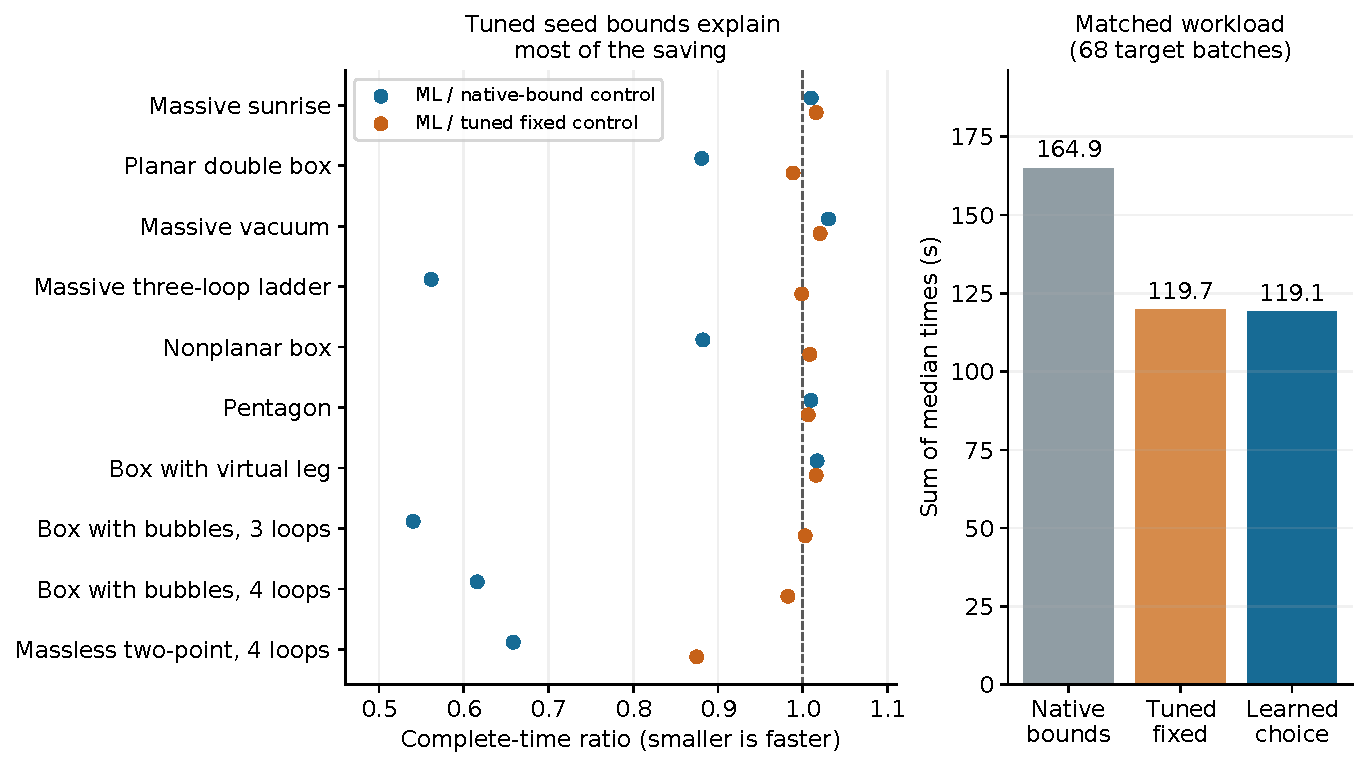
\includegraphics[width=\linewidth]{paper_figures/learned_bounds_times.pdf}
\caption{The left panel shows how the learned choice changes complete time for each graph; a ratio below one means a saving. The right panel shows the summed matched workload time. Both controls disable all learned choices. The graph labels refer to the explicit denominator definitions in the appendices.}
\label{fig:learned-bounds-times}
\end{figure}

The learned-to-control time ratios have descriptive 95\% intervals $[0.625, 0.885]$ against native bounds and $[0.980, 1.006]$ against the tuned fixed settings when whole graphs are resampled. Resampling repetitions within the fixed workload instead gives $[0.716, 0.727]$ and $[0.984, 1.006]$. The first calculation describes variation across this small graph collection; the second describes observed timing variation on these particular inputs. Neither interval proves a speedup on all integrals.

The summed generated-equation count changes from 2,029,994 under native bounds to 1,089,074 under learned choices, including equations from failed attempts. Average parameter loading and prediction take 7.067 and 0.836 milliseconds per learned request. Figure~\ref{fig:learned-bounds-effects} shows both the time ratios for each batch and the equation counts. The domain check and its time remain part of every learned request. The largest observed process-tree memory use is 946.8 MiB within the common limit.

\begin{figure}[!htbp]\centering
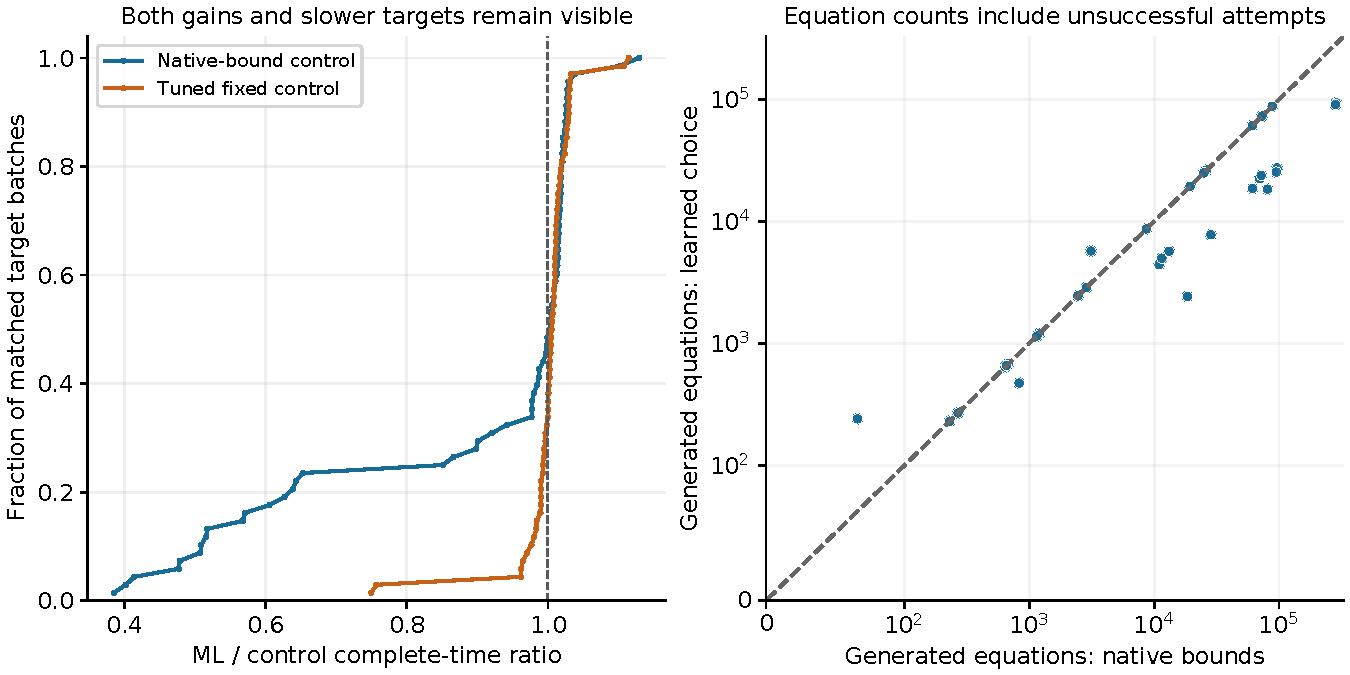
\includegraphics[width=\linewidth]{paper_figures/learned_bounds_effects.pdf}
\caption{Left: the distribution of batch time ratios retains every matched batch, including regressions. Right: generated equations under the learned and native-bound choices, with retries included. Points below the diagonal use fewer equations. The axes use a linear scale near zero and a logarithmic scale above 100 equations. Equation count explains part of the timing change but does not replace the complete-time measurement.}
\label{fig:learned-bounds-effects}
\end{figure}

Development, training-cost collection, validation, and their reference calculations take 1.37 hours of recorded calculation time, including 5.68 seconds for model fitting and selection. If future requests have the same mean saving as this matched workload, approximately 7295 requests would recover that cost relative to native bounds and 525989 relative to the fixed control. This extrapolation uses the measured workload and the derivation in Appendix~\ref{app:learned-bounds}; it is not a prediction for a different workload. The interval against the tuned fixed control includes equal time. Thus, this test establishes a saving from tuned seed settings but does not establish a reliable extra saving from learning which setting to use. The wider high-loop and symbolic coverage results retain the separate scope given in Section~\ref{sec:coverage}.

\subsection{Fresh application comparison}
A separate comparison starts a new application process for every request. It uses one fixed target pattern from each graph at the first reserved profile and three repetitions. The timer includes Python imports, input parsing, model loading, calculation, result storage, process exit, and coefficient checks. On 9 matched nontrivial batches, summed median time is 29.648 seconds for native bounds, 20.913 seconds for the previous published application, and 20.797 seconds for the new model. This is 29.9\% less time than the fresh native-bound application and 0.6\% less time than the previous application. The previous application retains its own validated portfolio and worker choices. Its comparison therefore measures the deployed workflow as a whole; the primary comparison above isolates the new learned choice.
